\documentclass{standalone}

\usepackage{graphics}
\usepackage[dvipsnames,svgnames]{xcolor}

\usepackage{tikz,pgf,pgfplots,circuitikz}
\pgfplotsset{compat=1.15}
\usepackage[compat=1.1.0]{tikz-feynhand}
\usetikzlibrary{intersections,arrows.meta,angles,calc,3d,decorations.pathmorphing}

\usepackage{amssymb,amsfonts,amsthm,mathtools}
\usepackage{physics,braket,bm}

\begin{document}  
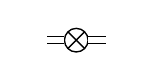
\begin{tikzpicture}[scale=1]
  \begin{feynhand}
    \vertex [particle] (a) at (0.5,0) {};
    \vertex [crossdot] (b) at (0,0) {};
    \vertex [particle] (c) at (-0.5,0) {};
    \draw [double distance=2pt] (a) to (b);
    \draw [double distance=2pt] (b) to (c);
  \end{feynhand}
\end{tikzpicture}
\end{document}
